\chapter{Rešerše elektronických komponent}
Základní návrh se skládá především z výběru bezdrátové komunikace, která je důležitou součástí Semaforu. Díky ní budou moci Semafory 
komunikovat mezi sebou, takže si například budou moci předávat informace o barvě, kterou svítí, nebo o stisku tlačítek apod. 

Další nedílnou součástí je mikrokontrolér, který řídí veškerou činnost každého Semaforu. U Semaforu je také nutné řešit způsob napájení,
takže i to je součástí návrhu.

Celkový návrh obsahuje také výběr senzorů doteku, zvukových a vizuálních signalizací a případných potřebných převodníků. 

\begin{figure}[!h]
  \begin{center}
    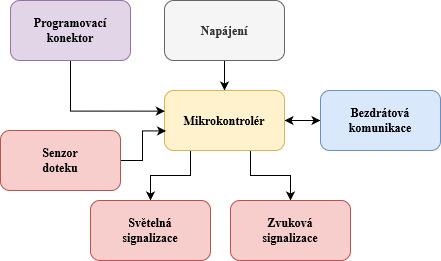
\includegraphics[scale=0.7]{obrazky/zakladni_blokove_schema.jpg}
  \end{center}
  \caption[Základní blokové schéma Semaforu]{Základní blokové schéma Semaforu.}
\end{figure}

\section{Bezdrátová komunikace}
Použití na táborech a outdoorových akcích vyřadilo z výběru drátovou komunikaci. K DPS by muselo být ještě velké množství kabelů 
o délce několika stovek metrů. Bezdrátová komunikace je z tohoto hlediska velmi praktická. Je to také moderní řešení 
náležící dnešní době. 

Jedním ze základních požadavků bylo, že jednotlivé DPS mezi sebou musí být schopny komunikovat. Proto byl nejdříve vybrán komunikační 
protokol a následně k němu přizpůsoben hardware. 

Práce tedy započala tím, že byla udělána rešerše existujících bezdrátových komunikačních protokolů a následně byly tyto protokoly 
mezi sebou porovnány. Vzhledem k použití na outdoorových akcích byl kladem důraz na komunikační vzdálenost, náročnost na výkon 
a také na dostupnost. 

Dalším požadavkem bylo bezdrátové nastavování, tedy připojení k Semaforu např. přes telefon a odeslání konfigurace. Nastavení hry,
která se hraje a např. čas, jak dlouho se bude hrát, nebo v kolika týmech, je tedy zapotřebí také dělat bezdrátově. 

\subsection{WiFi}
Komunikace pomocí WiFi sítě je jednou z nejznámějších a nejpoužívanějších bezdrátových komunikací užívaných širokou veřejností. 
WiFi je dnes na každém pracovišti, na veřejných místech i v každé domácnosti. Využívána je především pro připojení k internetu. 
Přes WiFi lze přenášet velké objemy dat vysokou rychlostí. Pracuje v pásmech v okolí frekvencí 2,4 GHz a 5,0 GHz s dosahem 
desítek až nižších stovek metrů \cite{Bezdrat_muni}. 

Výhody bezdrátové technologie WiFi jsou \cite{Bezdrat_muni}:
\begin{itemize}
  \item pracuje v bezlicenčním pásmu, 
  \item levná, 
  \item velmi rozšířená.
\end{itemize}

Nevýhody jsou \cite{Bezdrat_muni}:
\begin{itemize}
  \item omezený výkon (není možné pokrýt rozsáhlejší oblasti), 
  \item vyšší spotřeba energie.
\end{itemize}

\subsection{Bluetooth}
Bluetooth je také velmi rozšířenou technologií bezdrátové komunikace. Používá se na přenos dat na krátké vzdálenosti. V dnešní době 
rozšířené WiFi komunikace je její použití omezené. Běžně se využívala pro přenos fotografií z jednoho zařízení do druhého apod. V dnešní 
době se spíše využívá pro připojení bezdrátových periferií jako jsou bezdrátová sluchátka, myši a klávesnice. Tato technologie je zaměřena 
především na nízkou spotřebu, i proto je komunikační vzdálenost maximálně 100 metrů \cite{Bezdrat_muni}. V praxi jde ale o nižší desítky
metrů. Bluetooth je také technologií pro propojení pouze 2 zařízení, kde jedno je tzv. master a druhý tzv. slave \cite{Bezdrat_muni}. 
Jedno zařízení je tedy nadřazeno druhému. V případě telefonu a sluchátek je telefon nadřazený sluchátkům. 

Výhody bezdrátové technologie Bluetooth jsou \cite{Bezdrat_muni}:
\begin{itemize}
  \item nízká spotřeba.
\end{itemize}

Nevýhody jsou \cite{Bezdrat_muni}:
\begin{itemize}
  \item krátký dosah,
  \item možnost propojení pouze 2 zařízení.
\end{itemize}

\subsection{NFC}
NFC je jedna z novějších technologií, která je známá především při použití platby kartou. Jde tedy o přenos malých objemů dat na velmi krátkou 
vzdálenost, tj. do desítek centimetrů \cite{Bezdrat_muni}. NFC je technologií, kde stačí, aby pouze jedno zařízení mělo zdroj elektrické 
energie \cite{Bezdrat_muni}. Druhé zařízení se chová jako anténa, ze které je možné vyčíst informace \cite{Bezdrat_muni}. Například při 
platbě kartou v sobě karta nemá žádný zdroj energie, ale při přiložení k terminálu je pomocí elektromagnetické indukce vyčteno identifikační
číslo karty. Díky tomu je možné zaplatit. 

Výhody bezdrátové technologie NFC jsou \cite{Bezdrat_muni}:
\begin{itemize}
  \item rychlost,
  \item možnost interakce se zařízeními bez vlastního zdroje elektrické energie.
\end{itemize}

Nevýhody jsou \cite{Bezdrat_muni}:
\begin{itemize}
  \item velmi krátká komunikační vzdálenost,
  \item možnost komunikace pouze mezi dvěma zařízeními, 
  \item nízká rychlost přenosu,
  \item malý objem přenášených dat.
\end{itemize}

\subsection{Sigfox}
Sigfox je prvním celorepublikovým mobilním operátorem v České republice určený především pro IoT \cite{Sigfox_cz}. Využívá vysílače mobilního operátora T-Mobile, 
díky čemuž má pokrytí více než 90 \% území ČR \cite{Sigfox_Zooco}. Sigfox vysílá v nelicencovaném pásmu o frekvenci 868 MHz \cite{Sigfox_cz}. Jedná se o síť 
s velkým dosahem, 50 km na volném prostranství a až 5 km v zastavěných oblastech \cite{Sigfox_Zooco}.  

Jedná se o placenou službu, kdy až po zaplacení poplatku je poskytnuto připojení do sítě Sigfox \cite{Sigfox_Zooco}. Komunikace probíhá po 12 bajtových 
blocích s omezením na maximální počet 140 zpráv \cite{Sigfox_Zooco}. Síť je tedy určená především pro malý přenos dat např. pro dálkový odečet elektroměru 
nebo pro posílání dat ze senzorů. 

Výhody bezdrátové sítě Sigfox jsou \cite{Sigfox_cz} \cite{Sigfox_Zooco}:
\begin{itemize}
  \item nízké pořizovací náklady,
  \item nízká spotřeba energie (na baterie vydrží až 10 let),
  \item vysoké pokrytí území ČR,
  \item spolehlivost.
\end{itemize}

Nevýhody jsou \cite{Sigfox_cz}:
\begin{itemize}
  \item placená služba,
  \item omezený počet zpráv na den.
\end{itemize}

\subsection{LoRa}
LoRa je technologie, která moduluje data do elektomagnetických vln na fyzické vrstvě (rádio) umožňující komunikaci na velké vzdálenosti \cite{LoRa_eman}. 

LoRaWAN je komunikační protokol a architektura celé sítě \cite{LoRa_eman}. Je vhodná pro komunikaci mezi pohybujícími se předměty a její komunikace je 
zabezpečená \cite{LoRa_eman}. Tato síť má topologii hvězdy a pracuje v bezlicenčním pásmu \cite{LoRa_eman}. V České republice je povolená frekvence v pásmu 
okolo 868 MHz zdarma.

LoRa je technologie vyvinutá primárně pro IoT, takže je bezpečná a spolehlivá \cite{LoRa_IoT_PORT}. Zajišťuje také připojení na velkou vzdálenost (20 km na 
volném prostranství a 2 km v zastavěné oblasti) \cite{LoRa_IoT_PORT}. LoRa je také vyvinutá pro bateriová zařízení, takže je energeticky úsporná a na baterie
 vydrží zařízení až 10 let \cite{LoRa_IoT_PORT}.

Výhody bezdrátové technologie LoRa jsou \cite{LoRa_IoT_PORT}:
\begin{itemize}
  \item bezlicenční pásmo,
  \item spolehlivost,
  \item komunikace na velké vzdálenosti,
  \item obousměrná komunikace,
  \item dobrý poměr cena/výkon,
  \item energeticky úsporná.
\end{itemize}


\subsection{ZigBee}
ZigBee technologie je používána pro vytvoření malých sítí, kde může signál snadno přeskakovat z jednoho zařízení na druhé \cite{ZigBee_smart}.
Není přitom zapotřebí, aby bylo každé zařízení připojeno k internetu pomocí WiFi \cite{ZigBee_smart}. Pro komunikaci je ale zapotřebí centrální 
rozbočovač, který zajišťuje komunikaci mezi zařízeními \cite{ZigBee_smart}. Tato technologie je určena pro tvorbu rozsáhlejších bezdrátových sítí
s přenosem menšího objemu dat \cite{ZigBee_smart}. Jedná se o spolehlivou technologii s nenáročnou implementací a nízkou spotřebou elektrické energie 
\cite{ZigBee_smart}. Díky ZigBee může mít uživatel v jedné aplikaci zařízení 
od různých značek a výrobců, protože právě ZigBee zajišťuje jejich vzájemnou komunikaci \cite{ZigBee_smart}.

Technologie ZigBee je určeno primárně pro senzorové sítě v průmyslových aplikacích \cite{Bezdrat_muni}. Není vhodný pro práce s velkými objemy dat \cite{Bezdrat_muni}.
Pracuje v bezlicenčním frekvenčním pásmu \cite{Bezdrat_muni}.

Výhody bezdrátové technologie ZigBee jsou \cite{ZigBee_smart}:
\begin{itemize}
  \item nízká spotřeba elektrické energie,
  \item spolehlivost, 
  \item nenáročná implementace,
  \item pracuje v bezlicenčním frekvenčním pásmu. 
\end{itemize}

Nevýhodou je nutnost centrálního rozbočovače \cite{ZigBee_smart}.

\section{Světelná signalizace}
Jedním z nejdůležitějších požadavků na Semafor bylo, aby mohl svítit. Čím více možností jak svítit, tím bude využití při hrách a táborových 
programech různorodější. Pro světelnou signalizaci se nejvíce hodí použití LED. LED se výrabí programovatelné a neprogramovatelné. 

Neprogramovatelné LED jsou běžné LED, které mají 2 vývody - katodu a anodu. Barva LED je dána výrobou a každá LED má pouze jednu 
barvu. Přiložením daného prahového napětí na diodu v propustném směru se LED rozsvítí danou barvou. Velikost prahového napětí je dána
právě barvou LED. Běžně se pohybuje v rozmezí 1 až 2,5 V. Existují také RGB LED, které mají 4 vývody - 3 katody a společnou anodu. 
Přiložením napětí na konkrétní anodu je rozsvícena konkrétní barva. Při různě nastavené velikosti proudu lze regulovat jas LED 
a přiložením napětí na více LED lze svítit různými barvami a jejich odstíny. 

Programovatelné LED mají datový vstup a napájecí napětí není závislé na barvě LED. 
Barva je určována programem, taktéž její jas. To tedy znamená, že je zapotřebí je řídit 
pomocí MCU. Programovatelné LED typu WS2812C lze také spojovat za sebe, takže jsou všechny potřebné LED připojeny k jednomu pinu 
MCU \cite{WS2812C_dtsh}. Každá LED má pin pro vstupní napětí, GND, vstupní datový pin a výstupní datový pin. Typ inteligentních LED 
WS2812C je vhodný pro bateriová zařízení. Oproti častěji používanému typu WS2812B mají 3~$\times$~ menší spotřebu elektrické energie. 
Napájecí napětí těchto LED by se mělo pohybovat v rozmezí 4,5 až 5,5 V \cite{WS2812C_dtsh}. 

\section{Senzor doteku}
Senzory doteku jsou nezbytnými prvky pro ovládání Semaforu. Mohou sloužit pro přepínání módů, ovládání Semaforu jako takového nebo jako herní 
součást. Ve hře mohou plnit úlohu přepínače režimů hry, zadávání kódů, určování směru apod. 

Nejjednodušším a nejpoužívanějším senzorem doteku je tlačítko. 
Tlačítka mohou být realizována dvěma základními způsoby, mohou být elektromechanická, nebo dotyková kapacitní. 

Stisková plocha mechanického tlačítka je nevodivá, často plastová. Mechanické prvky jsou častým zdrojem problémů. Je tím často omezena i 
životnost celého výrobku. Mechanická konstrukce tlačítek je složitá a finančně nákladná. Mechanická tlačítka zároveň generují zákmity, které 
je nutno filtrovat nebo tvarovat do použitelné podoby. Nejjednodušším řešením je přidání kondenzátoru. Mechanická tlačítka existují typu NO 
a NC. 

Po zmáčknutí mechanického tlačítka typu NO jsou 2 kovové části tlačítka spojeny, tím dochází ke spojení elektrického obvodu 
a odpor smyčky je v ideálním případě nulový. Obvod je tedy sepnut. Když je tlačítko rozpojeno, tak je 
elektrický obvod přerušen a odpor smyčky je v ideálním případě nekonečný. Obvod je tedy rozpojen. U tlačítka typu NC je to naopak. Při stisku 
tlačítka je obvod rozepnut a při uvolnění stisku je obvod sepnut. 

\begin{figure}[!h]
  \begin{center}
    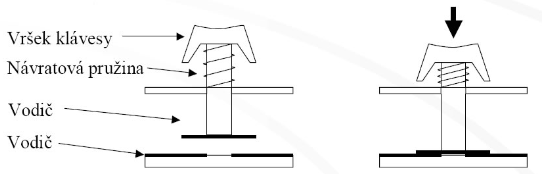
\includegraphics[scale=0.6]{obrazky/tlacitka_princip.png}
  \end{center}
  \caption[Princip mechanického tlačítka]{Princip mechanického tlačítka \cite{Mech_tl_princip}.}
\end{figure}

Výhody mechanických tlačítek jsou:
\begin{itemize}
  \item jednoduché připojení ke každému GPIO mikrokontroléru,
  \item odezva je samotný stisk tlačítka,
  \item fyzické rozpojení obvodu.
\end{itemize}

Kapacitní tlačítka jsou bez veškerých mechanických prvků, zároveň jsou jednoduchá a mají téměř neomezenou 
životnost. Jejich výstupní signál je bez jakýchkoli zákmitů nebo rušení. Kapacitní tlačítka lze snadno použít v mnoha aplikacích. 

Kapacitní tlačítka jsou tvořena měděnou vrstvou a nejsou nijak mechanicky namáhána. Tlačítko může být zmáčknuto i přes 
obal krabičky, a proto může být celé zařízení mechanicky odolné i voděodolné. 

Nevýhodou kapacitních tlačítek je, že nemají žádnou odezvu na dotyk. U mechanických tlačítek je odezvou samotný fyzický 
stisk tlačítka. U kapacitních tlačítek lze tento fakt vyřešit například rozsvícením LED nebo vibrační odezvou. Vibrační 
odezva může být realizována pomocí vibračního motoru. 

Některé mikrokontroléry nemají kapacitní vstupy, to znamená, že tlačítko nelze připojit přímo k GPIO pinu MCU \cite{ESP_C3_dtsh}. 
Buď musí být vybrán mikrokontrolér, který kapacitní vstupy má, nebo může být použit převodník, který má kapacitní vstupy a jeho 
výstupy poté mohou být připojeny k MCU. 

Výhody kapacitních tlačítek jsou:
\begin{itemize}
  \item kompaktnost,
  \item variabilita,
  \item vysoká spolehlivost,
  \item odolnost vůči šumu,
  \item možnost kompenzace rušivých elementů,
  \item cena. 
\end{itemize}

\subsection{Princip kapacitních dotykových tlačítek}
Základní princip je založen na měření změny kapacity. Měď, ze které je tlačítko vytvořeno má
nějakou vlastní kapacitu (kapacita samotné nosné desky) a po přiložení prstu je kapacita zvýšena o paralelně 
připojenou kapacitu přechodu tlačítka a prstu díky obsahu železa v krvi a vodivosti kůže \cite{PrincipKapTl}. 
Prst se tedy chová jako druhá uzemněná elektroda \cite{PrincipKapTl}. 

Kapacita snímače se tedy volí co nejmenší, aby přiložený prst vyvolal co nejvetší změnu kapacity. Ve snímači se vyskytuje
RC článek, kterého se mění doba nabíjení kondenzátoru a tím je možné detekovat stisk tlačítka \cite{PrincipKapTl}. 

\begin{figure}[!h]
  \begin{center}
    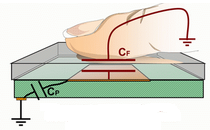
\includegraphics[scale=1]{obrazky/kapacitni_princip.png}
  \end{center}
  \caption[Princip kapacitního tlačítka]{Princip kapacitního tlačítka \cite{PrincipKapTl}.}
\end{figure}

\subsection{Návrh kapacitního dotykového tlačítka}
Tvar tlačítka nemá vliv na schopnost detekce dotyku \cite{PrincipKapTl}. Naopak velký vliv má plocha tlačítka, tloušťka
izolační vrstvy, a také vzdálenost jednotlivých tlačítek od sebe \cite{PrincipKapTl}. 

Čím větší je plocha tlačítka, tím je větší změna kapacity při dotyku a díky tomu je vytvořena lepší schopnost detekce 
dotyku \cite{PrincipKapTl}. S rostoucí tloušťkou izolační vrstvy se naopak schopnost detekce dotyku snižuje \cite{PrincipKapTl}.

Pokud jsou tlačítka příliš blízko u sebe, tak může docházet k jejich vzájemnému ovlivňování. Kvůli tomu pak může docházet k
detekci dotyku špatného tlačítka, nebo k falešné detekci dotyku. Z doporučení plyne, že pro dotyk prstu je vhodná velikost snímací 
plochu pro prst 13~$\times$~13 mm a jejich vzdálenost alespoň 5 mm od sebe \cite{PrincipKapTl}. Proti vzájemnému ovlivňování tlačítek
se používají uzemňovací meziplošky \cite{PrincipKapTl}. 

U kapacitních dotykových tlačítek je zapotřebí dbát na správné připojení k MCU. U vícevrstvých DPS nesmí pod tlačítky, ani pod přívody
k MCU, vést jiné dráhy, ani se zde nesmí vyskytovat jiné součástky \cite{PrincipKapTl}. Součástky nesmí být ani z vrchní, ani ze spodní 
strany DPS \cite{PrincipKapTl}. Přívody kapacitních tlačítek k MCU by měly být odstíněny pomocí GND signálu.

Voda a další nečistoty mění vlastní kapacitu tlačítka a může tak docházet k falešným stiskům tlačítka. Tento problém lze řešit softwarově. 
Lze využít faktu, že nečistoty působí dlouhodobě, ale stisk je krátkodobý \cite{PrincipKapTl}. Hodnotu vlastní kapacity tlačítka je tedy
možné softwarově upravovat v závislosti na aktuálních dlouhodobějších stavech a detekovat tak přesněji krátkodobý stisk tlačítka.

Pro odlišení tlačítek může být místo označeno například barevným potiskem. 

\section{Napájení}
Vzhledem k použití Semaforů při hrách na táborech byly možné pouze 2 způsoby napájení, pomocí powerbanky nebo baterií. 

Ve výběru baterií hraje velkou roli kapacita, napětí, velikost a cena. Požadavkem je také možnost nabíjení. Při použití na táboře by jinak musely být stále 
nové baterie v balení a musely by se neustále doplňovat a udržovat.

Moderní baterie jsou náchylné na přepólování, a proto není bezpečné, aby uživatel měnil baterie sám. Baterie by tedy musely být zabudované v zařízení 
bez možnosti výměny uživatelem. 

%kapacita baterie - jak dlouho by měla vydržet

Z nabíjecích baterií je možno vybírat z olověných baterií, Ni-MH, Li-Ion, Li-Pol a LiFePO4 baterií.

\subsection{Olověné baterie}
Maximální životnost olověné baterie je 300 až 400 cyklů \cite{LiFePO4_malina}. Nominální hodnota jednoho článku jsou 2 V \cite{olovene}. Jejich výroba je oproti
lithiovým bateriím velmi nenáročná \cite{olovene}. Jejich kapacita je závislá na konkrétním typu baterie \cite{olovene}. Tyto baterie jsou schopny dodávat vysoké
rázové proudy \cite{akumulatory}. Olověné akumulátory jsou velké a těžké a pro přenosná zařízení se tedy spíše nehodí. Hlavní nevýhodou je, že je potřeba je udržovat 
neustále v nabitém stavu \cite{olovene}. Její účinnost je závislá na odebíraném proudu a její životnost je závislá na teplotě \cite{olovene}. Mají dlouhou dobu 
nabíjení a obsahují toxické olovo, které je škodlivé pro životní prostředí \cite{olovene}. Olověné baterie se používají především v automobilech jako startovací 
baterie, v zabezpečovacích systémech atd. \cite{olovene}.

Výhody olověných baterií jsou \cite{olovene}:
\begin{itemize}
  \item cena,
  \item bezpečnost provozu,
  \item možnost recyklace,
  \item spolehlivost. 
\end{itemize}

\subsection{Ni-MH}
Baterie Ni-MH mají jmenovité napětí 1,2 V a jejich životnost je cca 1000 nabíjecích cyklů \cite{akumulatory}. Tyto akumulátory je zapotřebí před prvním použití, nebo po 
dlouhém nepoužívání, tzv. naformátovat \cite{akumulatory}. 
Jedná se o pozvolné nabíjení s nízkým nabíjecím proudem \cite{akumulatory}. Pro optimální použití je také doporučeno baterii nabít nejpozději 2 hodiny před použitím, aby se 
snížil vnitřní odpor Ni-MH baterie \cite{akumulatory}.

Výhody Ni-MH baterií jsou \cite{akumulatory}:
\begin{itemize}
  \item cena,
  \item malé samovybíjení,
  \item vysoká mechanická odolnost.
\end{itemize}

\subsection{Li-Pol}
Li-Pol baterie poskytují vysoké nabíjecí proudy a vysokou kapacitu a jejich jmenovité napětí je 3,7 V \cite{akumulatory}. Tyto baterie jsou citlivé na přesné nabití, a proto 
je možné používat pouze nabíječky určené pro nabíjení těchto baterií \cite{akumulatory}. Tyto nabíječky mají také balancer \cite{akumulatory}. Při skladování je také nutné 
udržovat nabití na 50 \% kapacity \cite{akumulatory}. Údržba takové baterie je proto velmi náročná a nehodí se do podobných zařízení, jako je Semafor. Při mechanickém poškození 
také hrozí požár těchto baterií \cite{akumulatory}.

Výhody Li-Pol baterií jsou \cite{akumulatory}:
\begin{itemize}
  \item vysoké nabíjecí proudy, 
  \item vysoká kapacita, 
  \item nízké samovybíjení,
  \item cena.
\end{itemize}

\subsection{Li-Ion}
Jmenovité napětí Li-Ion baterie je 3,6 V a její životnost je cca 2000 nabíjecích cyklů \cite{Li-Ion}. Tento typ baterie trpí tzv. stárnutím. Jde o proces, kdy ztrácí 
svoji kapacitu bez ohledu na používání \cite{Li-Ion}. Jejich kapacita je tedy závislá na reálném čase a na frekvenci používání. Jejich velkou nevýhodou je nebezpečí 
výbuchu při špatné manipulaci, např. zkratu apod. \cite{Li-Ion}. 

Výhody Li-Ion baterií jsou \cite{Li-Ion}:
\begin{itemize}
  \item nízká hmotnost,
  \item malé rozměry,
  \item vysoká kapacita,
  \item rychlé nabíjení,
  \item šetrné k životnímu prostředí. 
\end{itemize}

\subsection{LiFePO4}
LiFePO4 baterie mají jmenovité napětí v rozsahu 3 až 3,3 V \cite{LiFePO4_malina}. Její minimální provozní napětí je pak 2,5 V a maximální je 3,65 V \cite{LiFePO4_malina}.
LiFePO4 je dnes baterie známá jako nejbezpečnější, nejspolehlivější a nejstabilnější baterie obsahující lithium \cite{LiFePO4_malina}. Je to nejvhodnější baterie pro 
přenosná zařízení díky velmi dobrému poměru velikosti (hmotnosti) a kapacity. Její životnost je až 4$\times$ vetší než u baterie Li-Ion \cite{LiFePO4_malina}. Je také hodnocena
jako nejbezpečnější z dosud dostupných baterií \cite{LiFePO4_malina}. Baterie LiFePO4 mohou standardně dosáhnout životnosti až 7000 cyklů, to odpovídá cca 15 letům při bežném
používání \cite{LiFePO4_malina}. Článek LiFePO4 je teplotně stabilní, nehořlavý (ani při zkratu), netrpí samovybíjením, není toxický a nevytéká \cite{LiFePO4_malina}.

LiFePO4 baterie v dnešní době nahrazují baterie typu Li-Ion nebo Li-Pol.
Tyto bateriové články jsou vhodné především pro použití v elektromobilech, solárních a větrných elektrárnách, elektrokoloběžkách atd. 

Výhody LiFePO4 baterií jsou \cite{LiFePO4_smart}:
\begin{itemize}
  \item vysoký jmenovitý proud,
  \item minimální ztráty,
  \item krátká doba dobíjení,
  \item chemická odolnost,
  \item vyníkající poměr výkonu ku hmotnosti,
  \item životnost tisíce cyklů,
  \item snadnější recyklace,
  \item bez využití toxických prvků.
\end{itemize}


\section{Mikrokontrolér}
Mikrokontrolér je hlavním prvkem každého zařízení včetně Semaforu. Mikrokontrolérů existuje nespočetné množství od mnoha výrobců a při výběru je nutno brát v potaz
množství požadovaných parametrů a požadované periferie. 
Komunikační moduly pro bezdrátovou komunikaci se připojují nejčastěji pomocí $I^2C$ nebo UART rozhraní. Pro připojení zvukových a vibračních periferií jsou zapotřebí 
GPIO piny.

Cenu mikrokontroléru určuje především počet periferií, počet GPIO pinů a výpočetní výkon.

Známými výrobci mikrokontrolérů jsou Microchip, Motorola, NXP nebo \\STMicroelectronics. 

\newpage
Faktory ovlivňující výběr řídicího mikrokontroléru:
\begin{itemize}
  \item dostatečný počet GPIO pinů,
  \item dostatek paměti,
  \item nízká spotřeba,
  \item WiFi,
  \item ADC,
  \item $I^2C$,
  \item UART,
  \item cena.
\end{itemize}







